\include{dog16template}

\newcommand{\x}{\mathbf{x}}
\newcommand{\y}{\mathbf{y}}
\newcommand{\z}{\mathbf{z}}
\newcommand{\blambda}{\boldsymbol{\lambda}}
\newcommand{\bmu}{\boldsymbol{\mu}}
\newcommand{\bnu}{\boldsymbol{\nu}}
\usepackage{color}
\usepackage{tikz}
\usepackage{pgfplots}
\usetikzlibrary{positioning}
\usetikzlibrary{arrows}
\usepackage[margin=1in]{geometry}
\usepackage{multirow,booktabs}


\begin{document}
\lecture{3}{January 4, 2017}{Mohamad El laz}

%Notes
\section{Introduction}
%The goal of this lecture is to study a different distributed problem from what we have studied until now. 
In the previous lectures we considered examples where users wanted to transmit at a fixed rate, and were able to choose their transmission paths, their routes.

In this lecture, we study the case where routes are fixed, but users can change their transmission rate. This is the usual situation for TCP flows over the Internet. For this reason, we could title our lecture ``Bandwidth sharing over the Internet.''

\section{Problem definition}
Let us consider the case where a user wants to download some content from the Internet (Figure~\ref{fig:1}).

% Graph
\begin{figure}[!h]
	\centering
	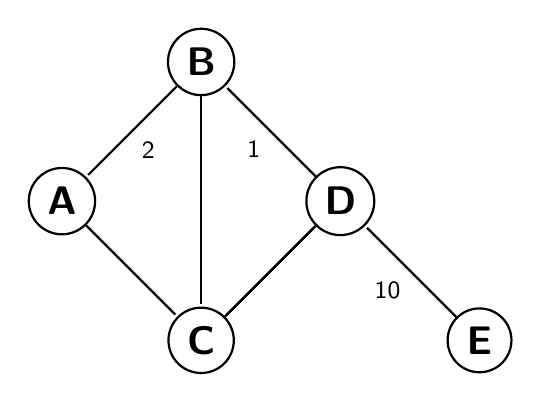
\begin{tikzpicture}[shorten >=1pt, auto, thick,
	auto,node distance=2.5cm,
	thick,main node/.style={circle,draw,font=\sffamily\Large\bfseries}]
	\node[main node] (1) {B};
	\node[main node] (2) [below left of=1] {A};
	\node[main node] (3) [below right of=2] {C};
	\node[main node] (4) [below right of=1] {D};
	\node[main node] (5) [below right of=4] {E};
	\path[every node/.style={font=\sffamily\small}]
	(1) edge node  {2} (2)
	edge node {} (3)
	(2) edge node {} (3)
    (3) edge node  {} (4)
	(4) edge node  {} (3)
	edge node {1} (1)
	(5)edge node {10} (4)	;
	\end{tikzpicture}
	\caption{server-client connection} \label{fig:1}
\end{figure}

In order to download some contents from the Internet, a connection might be established between the user and the server, this process is controlled by TCP (\textit{Transmission Connection Protocol}). TCP is a connection-oriented protocol, it determines how to break application data into packets that networks can deliver, sends packets to and accepts packets from the network layer, manages flow control, and handles retransmission of dropped or corrupted packets as well as acknowledgment of all packets that arrive.

In this example the route is fixed by the Internet provider. For the user, the faster its downloading rate, the better, but link capacities are limited and moreover they need to be shared with other users. We consider a first client (c1) downloading a file from the server on route A-B-D-E, a first constraint is that the download speed cannot exceed 1 Mbps, the capacity of link B-D.  The second constraint would be that another client (c2) is trying to download from the same source, e.g.~through route A-C-D-E or in any case he is sharing a common link (e.g. in Route C-B-D-E). To see how the Internet splits the downloading rate we will consider a general model.

\section{A general model for the problem}

We can consider that the ``happiness'' of a user is a function of his downloading rate. A very common way to model such happiness is by an increasing concave function (Figure~\ref{fig:2}):
\begin{itemize}
	\item Increasing as the higher the rate, the happier a user is.
	\item Concave because of the law of diminishing returns.
\end{itemize}

%law of diminishing return
\begin{remark}
	The law of diminishing return is a commonly used concept in the field of economy. For example, let us consider the diminishing marginal utility (happiness) of income, which means that as income increases, individuals gain correspondingly a smaller increase in happiness. To explain it better let us consider the example below.
	
	If you have zero income and gain 10\$ per day, this will improve your living standards significantly as you will be able to pay for basic necessity of life (i.e. food). 
	
	However, if you already gain 500\$� a day, an extra 10\$�� leads to a  smaller increase in utility (it does no��t significantly affect your standard of living and happiness).
	
	Now, if you are earning 15,000\$� a day, you would hardly notice an extra 10\$��. Therefore, then the marginal utility of an extra 10\$�� at this income level is very limited.
	
	The same idea is applied to the marginal happiness of users downloading from Internet, where the user is unhappy when there is no downloading rate and happier if the rate is higher. When having a twice faster connection, the user will be happier but not twice as much.
	
	Thus, as income increases, the extra marginal benefit to individuals declines.

\end{remark}

%Concave function
\begin{figure}[h]
	\centering
	\begin{tikzpicture}
	\begin{axis}[domain=-4:4, samples=1000,
	restrict y to domain=0:4,legend pos=north west]
	\addplot [color=blue]    {(ln(x)};
	\end{axis}
	\end{tikzpicture}
	\caption{An increasing concave function} \label{fig:2}
\end{figure}
\subsection{Solving the problem by the Lagrange multipliers method}
We will just identify the users as the routes  (one user corresponds to one route):
\begin{itemize}
	\item $R$ is the set of all routes/users.
	\item $E$ is the set of edges.
	\item $l \in r$ where link $l$ is a part of route $r$.
	\item $C_l$ is the capacity of link $l$ (the maximum traffic rate that $l$ can support).
	\item $U_r(x_r)$ is the utility of user $r$ for downloading at rate $x_r$.
\end{itemize}
Thus our objective is to maximize the sum of users happiness.

The optimization problem can be modeled as follows:
\begin{equation}
\begin{aligned}
& {\text{maximize}}
& &  \sum_{r \in R} U_{r}(x_{r}) \\
& \text{subject to}
& & \sum\limits_{r|l \in r} x_{r} \leq C_{l},\ \forall l \in E\\
&      &&  x_{r} \geq 0,\ \forall r \in R\\
\end{aligned}
\label{Max}
\end{equation}
We also denote $y_l=\sum\limits_{r | l \in r} x_r$.

For convenience, we also assume that $U_r(x_r)$ is strictly concave, and continuously differentiable on $[0,\infty)$. %, and satisfies $U'_r(0) = \infty$ and $U'_r(\infty) = 0$.

This is a problem for which we know that the Lagrangian is a necessary and sufficient condition (because the sum of concave functions is a concave function and the constraints are linear), so we can apply \textit{Theorem 2} of lecture 2a for concave maximization. We can also apply \textit{Theorem 1} of lecture 2a for convex minimization to the following problem:

\begin{equation}
\begin{aligned}
& {\text{minimize}}
& &  \sum_{r \in R} - U_{r}(x_{r}) \\
& \text{subject to}
& & \sum\limits_{r|l \in r} x_{r} \leq C_{l},\ \forall l \in E\\
&      &&  x_{r} \geq 0,\ \forall r \in R\\
\end{aligned}
\label{Min}
\end{equation}
The resulting Lagrangian function:
\begin{equation} 
L(\x, \bmu)= \sum_{r \in R} - U_{r}(x_{r}) + \sum_{l \in E} \mu_l \left(\sum_{r:l \in r} x_r - C_l\right) 
\end{equation}
When differentiated with respect to the rate on link $\bar r$:
\begin{equation}
\label{Derivative}
\begin{aligned}
\frac{\partial L}{\partial x_{\bar{r}}}= - U'_{\bar{r}}(x_{\bar{r}}) + \sum_{l \in \bar r} \mu_l
\end{aligned}
\end{equation}
$\x^*$ is a global minimizer iff:
\begin{enumerate}
	\item $x^*$ is feasible.
	\item There exists  $\mu^*_l  \geq 0$, such that $\nabla_\x L(\x^*,\bmu^*)^T (\x - \x^*) \ge 0,  \;\; \forall \x \in X$, where $X$ is the set of constraints we left out of the Lagrangian, i.e. $X = \{\x, x_r\ge0 \;\; \forall r\}$.
\end{enumerate}

The slack conditions are
 \begin{equation}
\label{e:mu}
\mu^*_l (\sum_{r:l \in r} x^*_r - C_l) = 0
\end{equation} 
One of the two factors is equal to zero, then
\begin{equation}
\mu^*_l
\begin{cases}
\ge 0  & \mbox{if the link is fully used},(\sum_{r:l \in r} x^*_r - C_l) = 0, \\
=0  &\mbox{if the link is under utilized}, (\sum_{r:l \in r} x^*_r - C_l) <0,
\end{cases}
\end{equation}


\subsubsection{The optimum value}
Let $x^*_{\bar r}$ be the optimum value of $x_{\bar r}$.

Observe that if $x^*_{\bar r} > 0$ we can consider feasible solutions $\x \in X$, whose $\bar r$-th component is larger or smaller than $x^*_{\bar r}$. We can find $\Delta x>0$ such that both $\x^* + \Delta x \mathbf{e}_{\bar r}$ and $\x^* - \Delta x \mathbf e_{\bar r}$ belong to $X$. Then, from the condition on the gradient of the Lagrangian, it follows:
$$ \frac{\partial L}{\partial x_{\bar r}}\bigg|_{\x^*, \bmu^*} \Delta x \geq 0,$$
$$ \frac{\partial L}{\partial x_{\bar r}}\bigg|_{\x^*, \bmu^*} (-\Delta x) \geq 0,$$
From these two results we can see that 
\begin{equation}
\label{e:equal}
\frac{\partial L}{\partial x_{\bar r}} =0,  \textrm{  if }x_{\bar r}^* >0.
\end{equation}

Instead if $x^*_{\bar r}=0$, it is only possible to increase it and we get:
\begin{equation}
\label{e:greater}
\frac{\partial L}{\partial x_{\bar r}}\bigg|_{\x^*, \bmu^*} \ge 0  \textrm{  if }x_{\bar r}^* =0
\end{equation}

From \eqref{e:equal}  we get that:
\begin{equation}
U'_{\bar{r}}(x^*_{\bar{r}})= \sum_{l \in {\bar r}} \mu^*_l, \textrm{  if }x_{\bar r}^* >0
\end{equation}
The structure is similar to the one we studied in the other examples. Again, we have that at the optimum, the marginal utility $U'_{\bar{r}}(x^*_{\bar{r}})$ should be equal to the sum over all the links in the route of the Lagrange multipliers associated to the link constraints. Moreover, the multipliers are \textit{equal to zero} over all the unused links and can be \textit{greater than zero} only over the utilized links. It is then natural to consider a Lagrange multiplier as the marginal congestion cost of the link, that expresses the damage that a user causes to other users transmitting over the same link. $\sum_{l \in {\bar r}} \mu^*_l$ is the marginal congestion cost of the route ${\bar r}$.


From  \eqref{e:greater}  we get that:
\begin{equation}
U'_{\bar{r}}(x^*_{\bar{r}})\leq \sum_{l \in {\bar r}} \mu^*_l,  \textrm{  if }x_{\bar r}^* =0
\end{equation}

In this case, user $\bar r$ does not transmit, because its 
marginal utility at $x_{\bar r}=0$ is smaller than the congestion cost on the route (and because of concavity it would be even smaller for positive transmission rates). An increase of its rate would cause a significant loss of utility to all the other users sharing one of the links on route $\bar r$. Therefore, user $\bar r$ gets nothing,  because the increase of his happiness is not worthy the increase of the congestion cost on the route and the decrease of other users' happiness.

\subsection{A first attempt to introduce dynamics}
Until now, we have characterized the equilibrium.
We would like to see also by which dynamics the system can converge to the optimum solution. The analysis above suggests the following possible operation: each link transmits to each user its current marginal congestion cost and users react to the current marginal congestion cost of the route by increasing/decreasing their rates.



In table \ref{tab:table1}, we consider the case of three users sharing the same congested link (capacity is equal to 10) according to the following simple discrete-time dynamics. Each user increases  its rate by one if the marginal congestion cost is null and decreases it if it is positive.
 Step by step, by increasing time, users increase their rate and the network tells them the cost of the congestion associated to the link. Once the congestion is reached ($>0$), the network tells the users to decrease their rate and the process repeats itself, without never reaching the equilibrium. 
This example suggests that an (ON-OFF) congestion signal, where links only reveal if there is or not congestion, may not be lead the system to converge to the optimum. 

In the next section we will slightly modify the problem by looking at a system for which links provide feedback even before being completely utilized. We will see a particular dynamic that actually converges to the solution of the optimum.

%table
\begin{table}[h!]
	\centering
	\caption{Congested link}
	\label{tab:table1}
	\begin{tabular}{ccccc}
		\toprule
		Time & User $r_1$  & User $r_2$ & User $r_3$ & Congestion\\
		\midrule
		0 & 0 & 0 & 0 &0\\
		1 & 1 & 1 & 1&0\\
		2 & 2 & 2 & 2 &0\\
		3 & 3 & 3 & 3 &0\\
		4 & 4 & 4 & 4 & {$>0$}\\
		3 & 3 & 3 & 3 &0\\
		4 & 4 & 4 & 4 & {$>0$}\\
		... & ... & ... & ... &...\\
		\bottomrule
	\end{tabular}
\end{table}

\section{A relaxed version of the problem}

%We would like to study a dynamic system and see how can a TCP controller actually maximize a given problem adapting the rate continuously.

What we have seen until now is the system where  the cost of congestion is zero up to where we have no congestion, then positive when we have congestion. But it is not the best way for a dynamic system, it would be  better if we have a situation where we already pay something when we approach congestion.We look at a slightly different problem where we can even violate the constraints on the capacity but at the same time we will have an additional cost related to the congestion.

Let us imagine that for every link there is some cost $M_l(y_l)$ (figure)
This function should be increasing (increases with the rate), strictly convex (because it should grow faster when we arrive to $C_l$) and  non negative. Note that we could assume that $M_l(y_l)$ has a vertical asymptote for $y_l=C_l$, but we will consider that $M_l(y_l)$ has finite value also for $y_l\ge C_l$. This will allow us to take into account the possibility that the traffic on a link may temporarily exceed the link capacity (this extra traffic may be accommodated by link buffers).

\begin{figure}[h]
	\centering
	\begin{tikzpicture}
	\begin{axis}[domain=-5:5,
	restrict y to domain=-5:5,xlabel=$y_l$,ylabel=$M(y_l)$, legend pos=north west]
	\addplot [color=blue]    {*exp(x)};
	\addplot[mark=*] coordinates {(0,0)} node[pin=0:{$(C_l)$}]{} ;
	\end{axis}
	\end{tikzpicture}
	\caption{An increasing convex function [RATES CANNOT BE NEGATIVE]} \label{fig:3}
\end{figure}

Another technical condition it that this function should grow faster than the utility. This guarantees that the optimal solution of the problem below corresponds to finite rate values. For this reason, we introduce the following condition:
 
\begin{equation}
\lim_{x\to\infty} U_r(x_r)-M_l(x_r)=-\infty,\ \forall r \in R\\, \ \forall l \in E\\
\end{equation}


So now, we consider a relaxed version of our initial problem in which we have no more hard constraint but a softer constraint transformed into a cost.
\begin{equation}
\begin{aligned}
& \underset{\x , \y }{\text{maximize}}
& &  \sum_{r \in R} U_{r}(x_{r})- \sum_{l \in E} M_{l}(y_{l})\\
& \text{subject to}
& & \ y_l=\sum\limits_{r | l \in r} x_r \\
&      &&  x_{r} \geq 0,\ \forall r \in R\\
\end{aligned}
\label{Max2}
\end{equation}
Where $M_l(y_l)$ is the cost of congestion on link $l$.

So let us write again the Lagrangian as:
\begin{equation} 
L(\x,\y,\bnu)= -\sum_{r \in R} U_{r}(x_{r}) + \sum_{l \in E} M_l(y_l)- \sum_{l \in E} \nu_l\left(y_l - \sum_{r:l \in r} x_r\right) 
\end{equation}
Then the derivatives are:
\begin{equation}
\label{e:M}
\begin{cases}
\frac{\partial L}{\partial y_{\bar{l}}}=M'_{\bar{l}}(y_{\bar{l}})-\nu_{\bar{l}}\\\\
\frac{\partial L}{\partial x_{\bar{r}}}=-U'( x_{\bar{r}}) + \sum_{l \in \bar{r}} \nu_l
\end{cases}
\end{equation}

Following the same reasoning as in the last lesson we have:

\begin{equation}
\begin{aligned}
\frac{\partial L}{\partial x_{\bar r}}\bigg|_{\x^*,\y^*,\nu^*}
\begin{cases}
= 0 & \mbox{if } x_{\bar r}^* \geq 0,\\
\geq0 & \mbox{if } x_{\bar r}^* = 0,
\end{cases}
\end{aligned}
\end{equation}

So from \eqref{e:M} we get:
$$\nu^*_{\bar l}=M'_l(y^*_{\bar l})$$
and
\begin{equation}
\label{e:equilibrium}
\ U'(x^*_{\bar r})
\begin{cases}
= \sum_{l \in {\bar r}} \nu^*_l  & \mbox{if } x^*_{\bar r} > 0,\\ 
\leq \sum_{l \in {\bar r}} \nu^*_l & \mbox{if }x^*_{\bar r} = 0.
\end{cases}
\end{equation}
As above, at the equilibrium on each route the marginal utility is equal to the total marginal congestion cost of the route. In this case the marginal congestion cost of a link is expressed by $M'_l(y_l)$.
Because of the convexity of $M_l(y_l)$, the marginal congestion cost is increasing in the traffic on the link.

\subsection{Convergence}
Now we can study a new system dynamics. 
Let $x_r(t)$ and $y_l(t)$ denote respectively the transmission rate along route $r$ and the traffic on link $l$ at time $t$.
We can think that user $r$ increases/decreases its rate proportionally to the difference between his marginal utility and the marginal congestion cost along the route:
\begin{equation}
\label{e:dynamics}
\frac{dx_r}{ dt}=k_r(U'(x_r(t)) - \sum_{l \in { r}} M'_l(y_l(t) )   )
\end{equation}

Where do we expect this system to converge? Immagine that the system stops at a given configuration. Let $\hat x_r$ and $\hat y_l$ denote the corresponding quantities. If this is an equilibrium, then \eqref{e:dynamics} should predict that the rates do not change anymore, but from the right hand side of the equation, it follows:
 $U'(\hat x_r)= \sum_{l \in r} M'_l(\hat y_l)$
 
The equilibrium of the dynamics indicated by \eqref{e:dynamics} corresponds then to the optimal solution of our optimization problem.
We can conclude that, if the dynamics stop, then they stop at a global optimizer.

So if everyone adapts his rate according to \eqref{e:dynamics} and the system stops, this will be at the optimum. In fact this approach is not rigorous because we actually do not know if it will stop.

Next we show that the congestion avoidance algorithm of TCP, due to Jacobson (1988), can be described in this framework.

\section{Modeling TCP}
We start describing a simplified operation for TCP.

Let $T_r$,  be the round-trip time along route $r$, i.e. the time between a source sending a packet and the source receiving an acknowledgement. The source maintains a window (of size cwnd) of packets that have been sent but not yet acknowledged. The transmission rate $x$ can then be calculated as cwnd/$T_r$. During one round-trip time $T_r$, the source should receive cwnd acknowledgements (then one every $T_r$/cwnd). If a given  acknowledgement is received, then cwnd is increased by 1/cwnd. If the acknowledgement is not received, cwnd is halved.

Let $p_r$ be the packet loss probability over route $r$. During the time $T_r$/cwnd, cwnd increases of 1/cwnd with probability $1-p_r$ and decreases of cwnd/2 with probability $p_r$. Similarly, the instantaneous rate will change as follows:
\begin{itemize}
	\item if there is no packet loss (and then with probability $1-p_r$), it will increase by $ \dfrac{1/cwnd}{T_r}$
	\item if pachet loss  (and then with probability $p_r$), it will decrease by $-\dfrac{cwnd}{2T_r}$.
\end{itemize}

The expected change of the rate is then $\Delta x_r = \dfrac{1/cwnd}{T_r} (1-p_r)- \dfrac{cwnd}{2T_r} p_r$. The evolution of the rate can then be approximated as follows:
\begin{equation}
\label{eq:der}
\begin{split}
\dfrac{dx_r}{dt}&=\dfrac{\Delta x_r}{T_r/cwnd} \\
&=\dfrac{cwnd}{T_r}\left(\dfrac{1/cwnd}{T_r}(1-p_r)- \dfrac{cwnd}{2T_r} p_r \right)\\
&=\dfrac{1}{T_r^2}(1-p_r)-\dfrac{cwnd^2}{2T_r^2} p_r\\
&=\dfrac{1}{T_r^2}-p_r \left(\dfrac{1}{T_r^2}+\dfrac{x_r^2}{2}\right)\\
&=\dfrac{1}{T_r^2}\left(1-p_r(1+\dfrac{x_r^2 T_r^2}{2})\right)\\
&=\dfrac{1+\dfrac{x_r^2 T_r^2}{2}}{T_r}\left(\dfrac{1}{1+\dfrac{x_r^2 T_r^2}{2}}-p_r\right)
\end{split}
\end{equation}
By a comparison with \eqref{e:dynamics}, the first term in \eqref{eq:der} plays the same role of $k_r>0$, that is a parameter affecting the speed of convergence, but not its direction.

The term $1/\left(1+\dfrac{x_r^2 T_r^2}{2}\right) $ corresponds to the marginal utility $U'_r(x_r)$ that a user gets from transmitting at rate $x_r$. By integrating, we obtain then that:
\begin{equation}
U_r(x_r)=\dfrac{\sqrt{2}}{T_r}\arctan \dfrac{x_r  T_r}{\sqrt{2}}
\end{equation}

The term $p_r$ should correspond to the marginal cost of congestion on route $r$. $p_r$ is the packet loss probability, that is indeed an indication of congestion. We would like the marginal congestion cost on a route to be expressed as sum of link costs, but the probability to lose a packet on a route is not the sum of probability to lose the packet over all links. For example consider a route $r$ with 3 links. The probability of losing a packet is:
\begin{equation}
\label{eq:prob}
p_r=1-(1-p_1)(1-p_2)(1-p_3)
\end{equation}
But if the probability to lose a packet is not high then \eqref{eq:prob} would be equal to:
\begin{equation}
p_r\approx1-1+p_1+p_2+p_3=p_1+p_2+p_3
\end{equation}

If we assume that the network is working with low packet loss probabilities, then we can identify:
\begin{equation}
M'_l(y_l)=p_l(y_l),
\end{equation}
from which we obtain that
\begin{equation}
M_l(y_l)=\int_{0}^{y_l} p_l(t) dt
\end{equation}



We conclude that all TCP sources together are solving the following problem:
\begin{equation}
\begin{aligned}
& {\text{maximize}}
& &  \sum_{r \in R} \dfrac{\sqrt{2}}{T}\arctan \dfrac{(x_r)(T)}{\sqrt{2}}- \sum_{l \in E} \int_{0}^{y_l} p_lt) dt\\
& \text{subject to}
& & y_{l} = \sum\limits_{r|l \in r} x_{r},\ \forall l \in E\\
&      &&  x_{r} \geq 0,\ \forall r \in R\\
\end{aligned}
\end{equation}

This is the global optimization problem that TCP is solving in a distributed way. We see that TCP (or at least our differential equation model of it) is behaving as if it is maximizing the sum of user utilities, subject to a cost function penalizing proximity to the capacity constraints.
We saw how every TCP source cares only of packet losses along its path. The specific optimization problem solved by TCP sources is difficult to justify, but TCP congestion control was originally proposed to avoid congestion collapses and not to solve a meaningful optimization problem. Later, once this optimization framework had been recognized, other congestion control mechanisms have been engineered. In theory these other mechanisms are better than TCP, but they were not widely adopted. The problem is that we cannot start from scratch. In general if we could restart the Internet, we know how to do it better. But we cannot switch off all the transmitting computers and start them with the new congestion protocols. All the new protocols suffer for the fact that they are less aggressive than TCP, and then they perform worse in a heterogeneous scenario where other users still adopt TCP. Some of these protocols are now used for inter-machine communication inside data centers.

\begin{thebibliography}{alpha}
	
	\bibitem{Kel14} Frank Kelly and Elena Yudovina,
	\newblock Stochastic Networks.
	\newblock {\em Cambridge Press}, 2014.
	
\end{thebibliography}



\end{document}



























































